\section{Наблюдатель полного порядка}
Рассмотрим систему:
\begin{equation}
    \begin{array}{ll}
        \dot{x} = Ax\\
        y = Cx
    \end{array}
\end{equation}
где
\begin{equation}
    \begin{array}{ccc}
        A = \begin{bmatrix}
            -40 & 16 & 9 & 7 \\ 
            -64 & 25 & 14 & 12 \\ 
            -26 & 11 & 7 & 3 \\ 
            -48 & 18 & 14 & 8
        \end{bmatrix}, & 
        C = \begin{bmatrix}
            -3 \\ 2 \\ -2 \\ 1
        \end{bmatrix}^T
    \end{array}
\end{equation}
\subsection{Наблюдаемость собственных чисел}
Для определения наблюдаемости собственных чисел рассмотрим вещественную Жорданову форму системы:
\begin{equation}
    \begin{array}{ll}
        \dot{\hat{x}} = P^{-1}AP\hat{x}\\
        \hat{y} = C\hat{x}
    \end{array}
\end{equation}
Где $P$ -- матрица собственных векторов матрицы $A$, а $\hat{x} = P^{-1}x$.
\begin{equation}
    \begin{array}{ccc}
        \begin{bmatrix}
            -0.00  & -2.00  & 0.00  & 0.00 \\ 
            2.00  & 0.00  & 0.00  & 0.00 \\ 
            0.00  & 0.00  & -0.00  & -3.00 \\ 
            0.00  & 0.00  & 3.00  & 0.00 \\ 
        \end{bmatrix}, &
        P = \begin{bmatrix}
            1.14  & -0.05  & 1.13  & 0.14 \\ 
            1.74  & -0.22  & 1.84  & 0.14 \\ 
            0.87  & -0.11  & 0.71  & 0.00 \\ 
            1.41  & 0.00  & 1.41  & 0.00 \\ 
        \end{bmatrix}, & 
        C_j =\begin{bmatrix}
            -0.27 \\ -0.05  \\ 0.28  \\ -0.14 \\ 
        \end{bmatrix}^T
    \end{array}
\end{equation}
Таким образом, система является полностью наблюдаемой. 

\subsection{Наблюдатель полного порядка}
Рассмотрим наблюдатель полного порядка:
\begin{equation}
    \begin{array}{ll}
        \dot{\hat{x}} = A\hat{x} + L(\hat{y} - y) \\
        \hat{y} = C\hat{x}
    \end{array}
\end{equation}
И схему его моделирования в среде Simulink. Схема моделирования представлена на рисунке \ref{fig:scheme2}.
\begin{figure}[ht!]
    \centering
    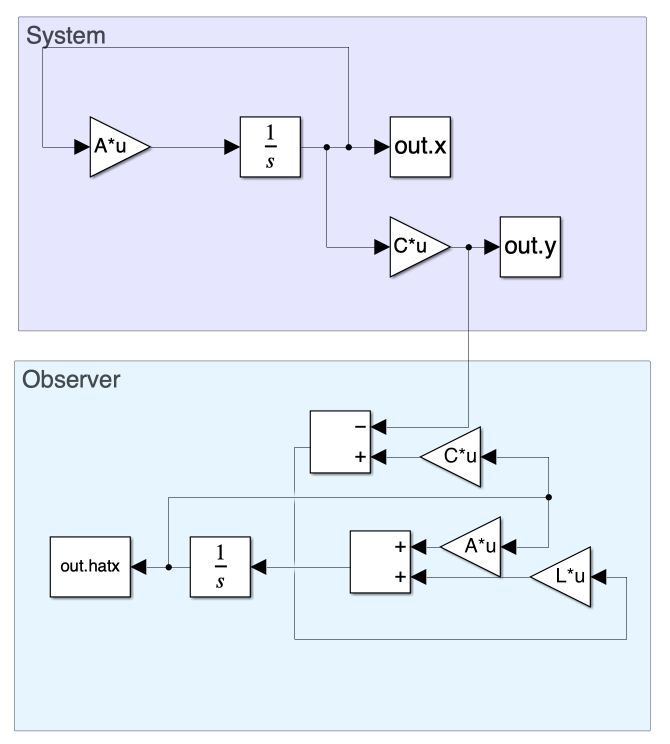
\includegraphics[width=0.6\textwidth]{media/scheme2.png}
    \caption{Схема моделирования системы с наблюдателем полного порядка}
    \label{fig:scheme2}
\end{figure}

\subsubsection{Подбор спектра нааблюдателя}
Рассмотрим следующие варианты спектра наблюдателя:
\begin{enumerate}
    \item  $\sigma_1 = \{-1, -1, -1, -1\}$
    \item $\sigma_2 = \{-1, -10, -100, -100\}$
    \item $\sigma_3 = \{-1\pm2j, -1\pm3j\}$
\end{enumerate}
Для каждого из спектров найдем вектор $L_i$ такой, чтобы спектр наблюдателя $\sigma(A + L_iC) = \sigma_i$. 
Если такой вектор существует, то существует и матрица перехода $V$ такая, что $A + L_iC = V^{-1}\Gamma_iV$, где 
$\Gamma_i$ -- матрица с нужным спектром. 
Зададимся матрицей $\Gamma_1$ со спектром $\sigma_1$: 
\begin{equation}
    \Gamma_1 = \begin{bmatrix}
        -1 & 1 & 0 & 0\\
        0 & -1 & 1 & 0\\
        0 & 0 & -1 & 1\\
        0 & 0 & 0 & -1
    \end{bmatrix}\quad \sigma(\Gamma_1) = \{-1, -1, -1, -1\}
\end{equation}
Запишем и решим уравнение Сильвестра с помощью покета \texttt{cvx}: 
\begin{equation}
    \begin{array}{ll}
        \Gamma_1 V - VA = YC\\
        Y = VL_1
    \end{array}
\end{equation}
где $Y$ -- такая матрица, чтобы пара $(\Gamma_1, Y)$ была наблюдаемой. Решив, получим матрицу $L$:
\begin{equation}
    L_1 = \begin{bmatrix}
        -33.23 \\ 
        -53.40 \\ 
        -22.57 \\ 
        -42.03 \\ 
    \end{bmatrix}
\end{equation}
Спектр системы $A + L_1C$ при этом оказывается $\{-1.023, -1\pm0.0023j, -0.997\}$, что практически 
полностью совпадает с требуемым спектром. 

Те же самые вычисления проведем для спектра $\sigma_2$:
\begin{equation}
    L_2 = \begin{bmatrix}
        161410.88 \\ 
        255685.22 \\ 
        116505.54 \\ 
        205662.28 \\ 
    \end{bmatrix}
\end{equation}
Спектр системы $A + L_2C$ при этом оказывается $\{-1, -10, -99.99, -100.0057\}$, что практически
полностью совпадает с требуемым спектром.

И для спектра $\sigma_3$:
\begin{equation}
    L_3 = \begin{bmatrix}
        11.93 \\ 
        16.80 \\ 
        7.67 \\ 
        13.53 \\ 
    \end{bmatrix}
\end{equation}
Спектр системы $A + L_3C$ при этом оказывается полностью равен требуемому спектру $\sigma_3$. 

Таким образом, для всех трех спектров существует такая матрица $L$, что спектр системы $A + LC$ совпадает с требуемым. 

\subsection{Моделирование}
Проведем моделирование каждой из систем с наблюдателем полного порядка с начальными условиями $x(0) = \begin{bmatrix} 1 & 1 & 1 & 1 \end{bmatrix}^T$ 
для самой системы и $\hat{x}(0) = \begin{bmatrix} 2 & 0 & 0 & -1 \end{bmatrix}^T$ для наблюдателя.

Результаты моделирования для первого спектра $\sigma_1$ представлены на рисунках \ref{fig:task2_x1_1}, \ref{fig:task2_x2_1}, \ref{fig:task2_x3_1} (состояния системы), и \ref{fig:task2_diff_1} (ошибка наблюдателя).
\begin{figure}[ht!]
    \centering
    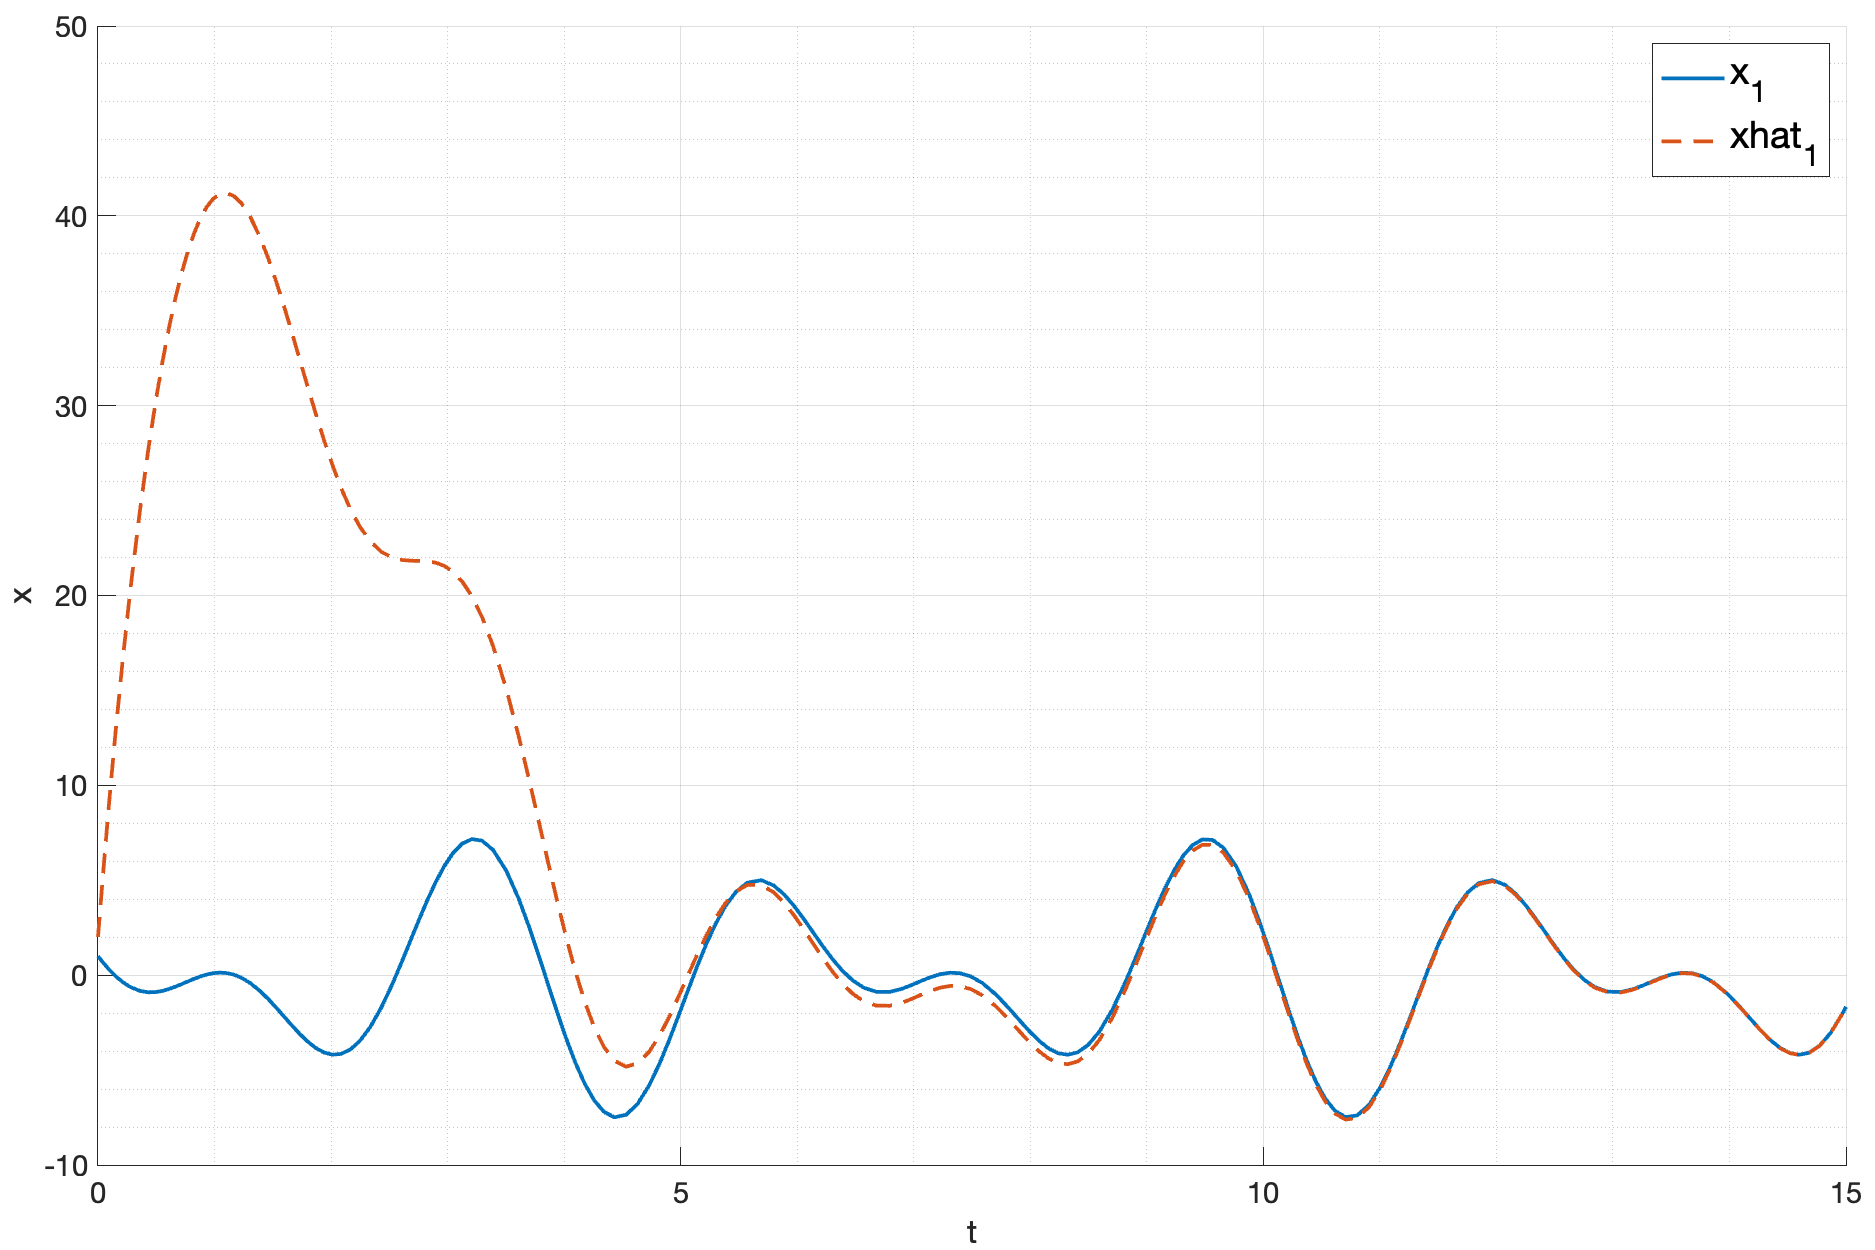
\includegraphics[width=\textwidth]{media/plots/task2_x1_1.png}
    \caption{Состояние системы $x_1$ с наблюдателем полного порядка для спектра $\sigma_1$}
    \label{fig:task2_x1_1}
\end{figure}

\begin{figure}[ht!]
    \centering
    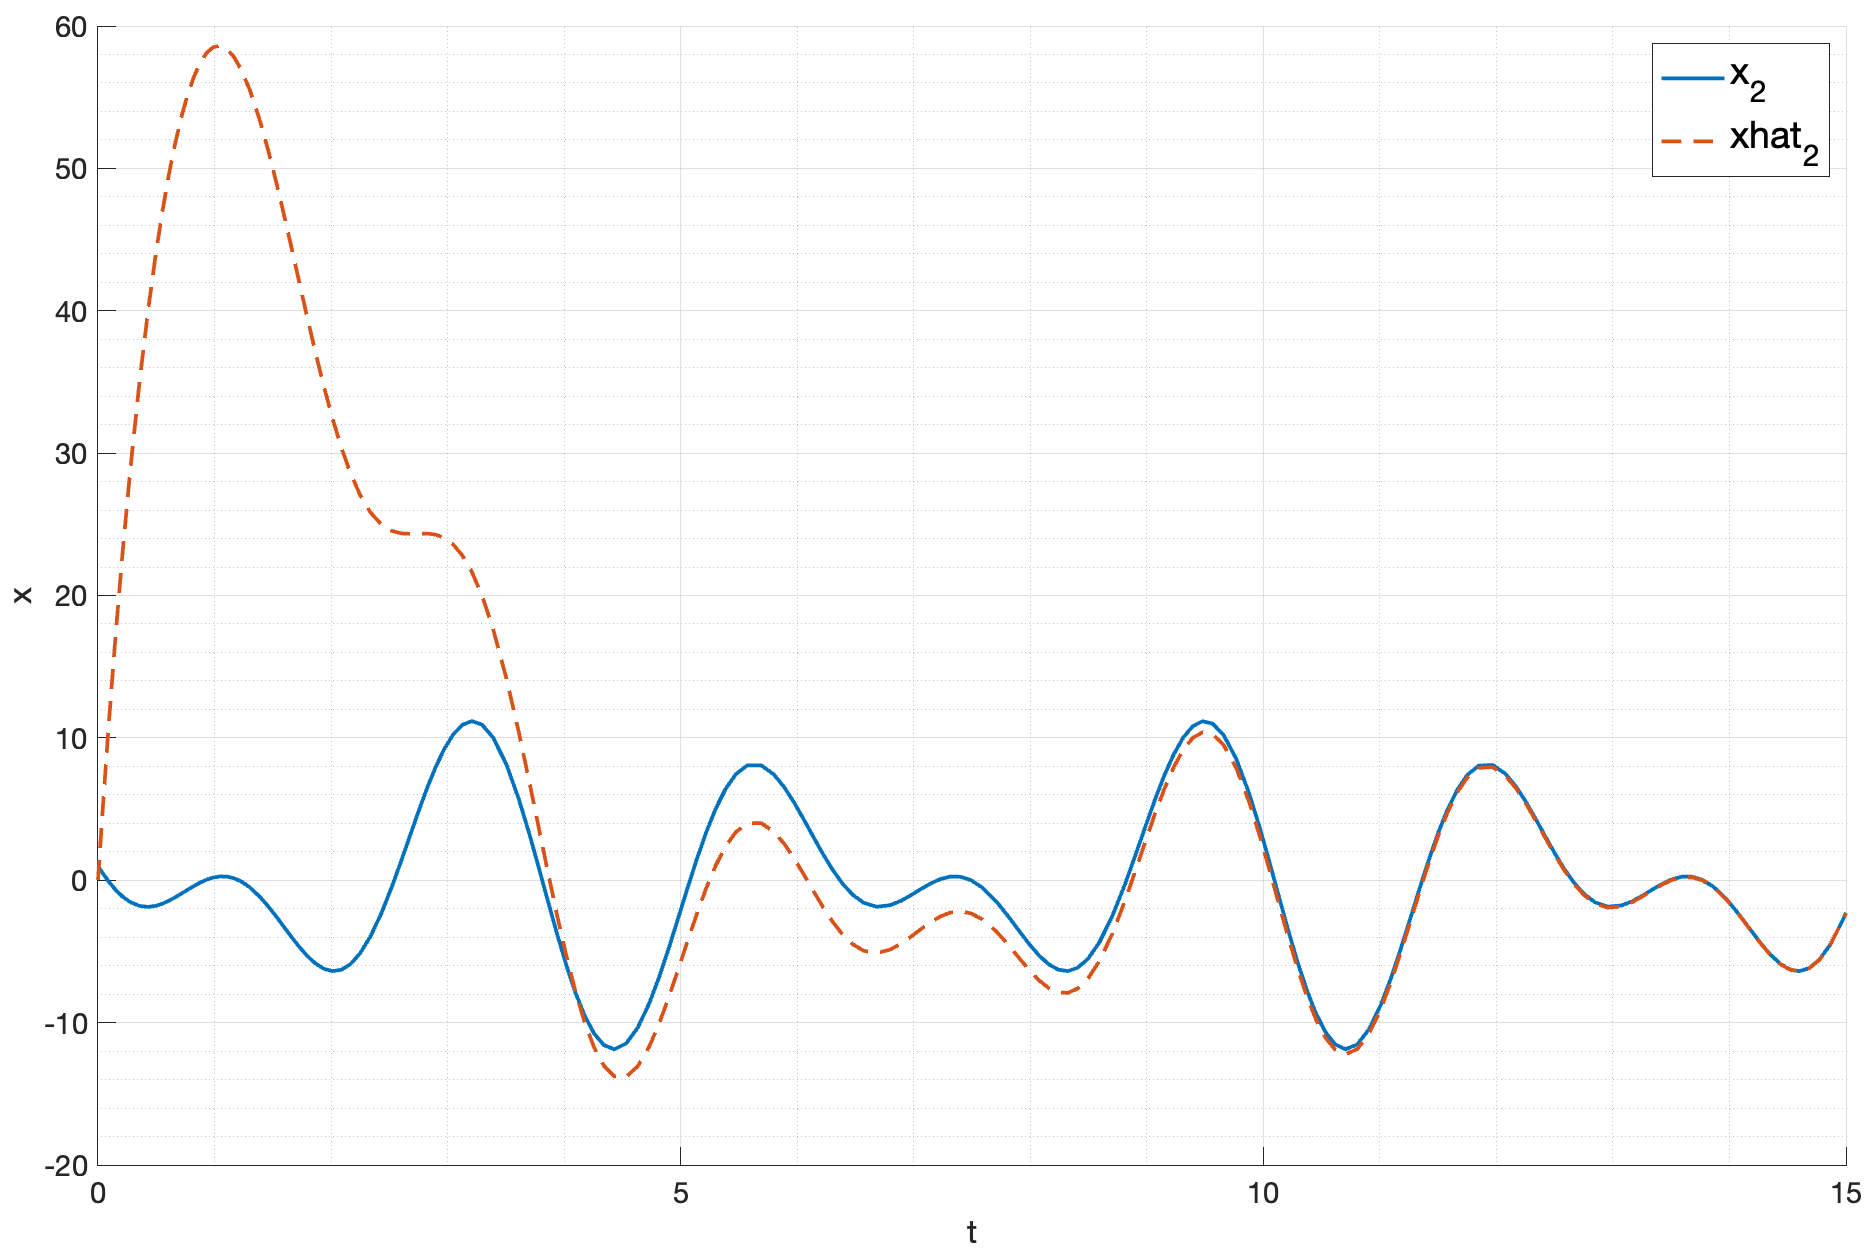
\includegraphics[width=\textwidth]{media/plots/task2_x2_1.png}
    \caption{Состояние системы $x_2$ с наблюдателем полного порядка для спектра $\sigma_1$}
    \label{fig:task2_x2_1}
\end{figure}

\begin{figure}[ht!]
    \centering
    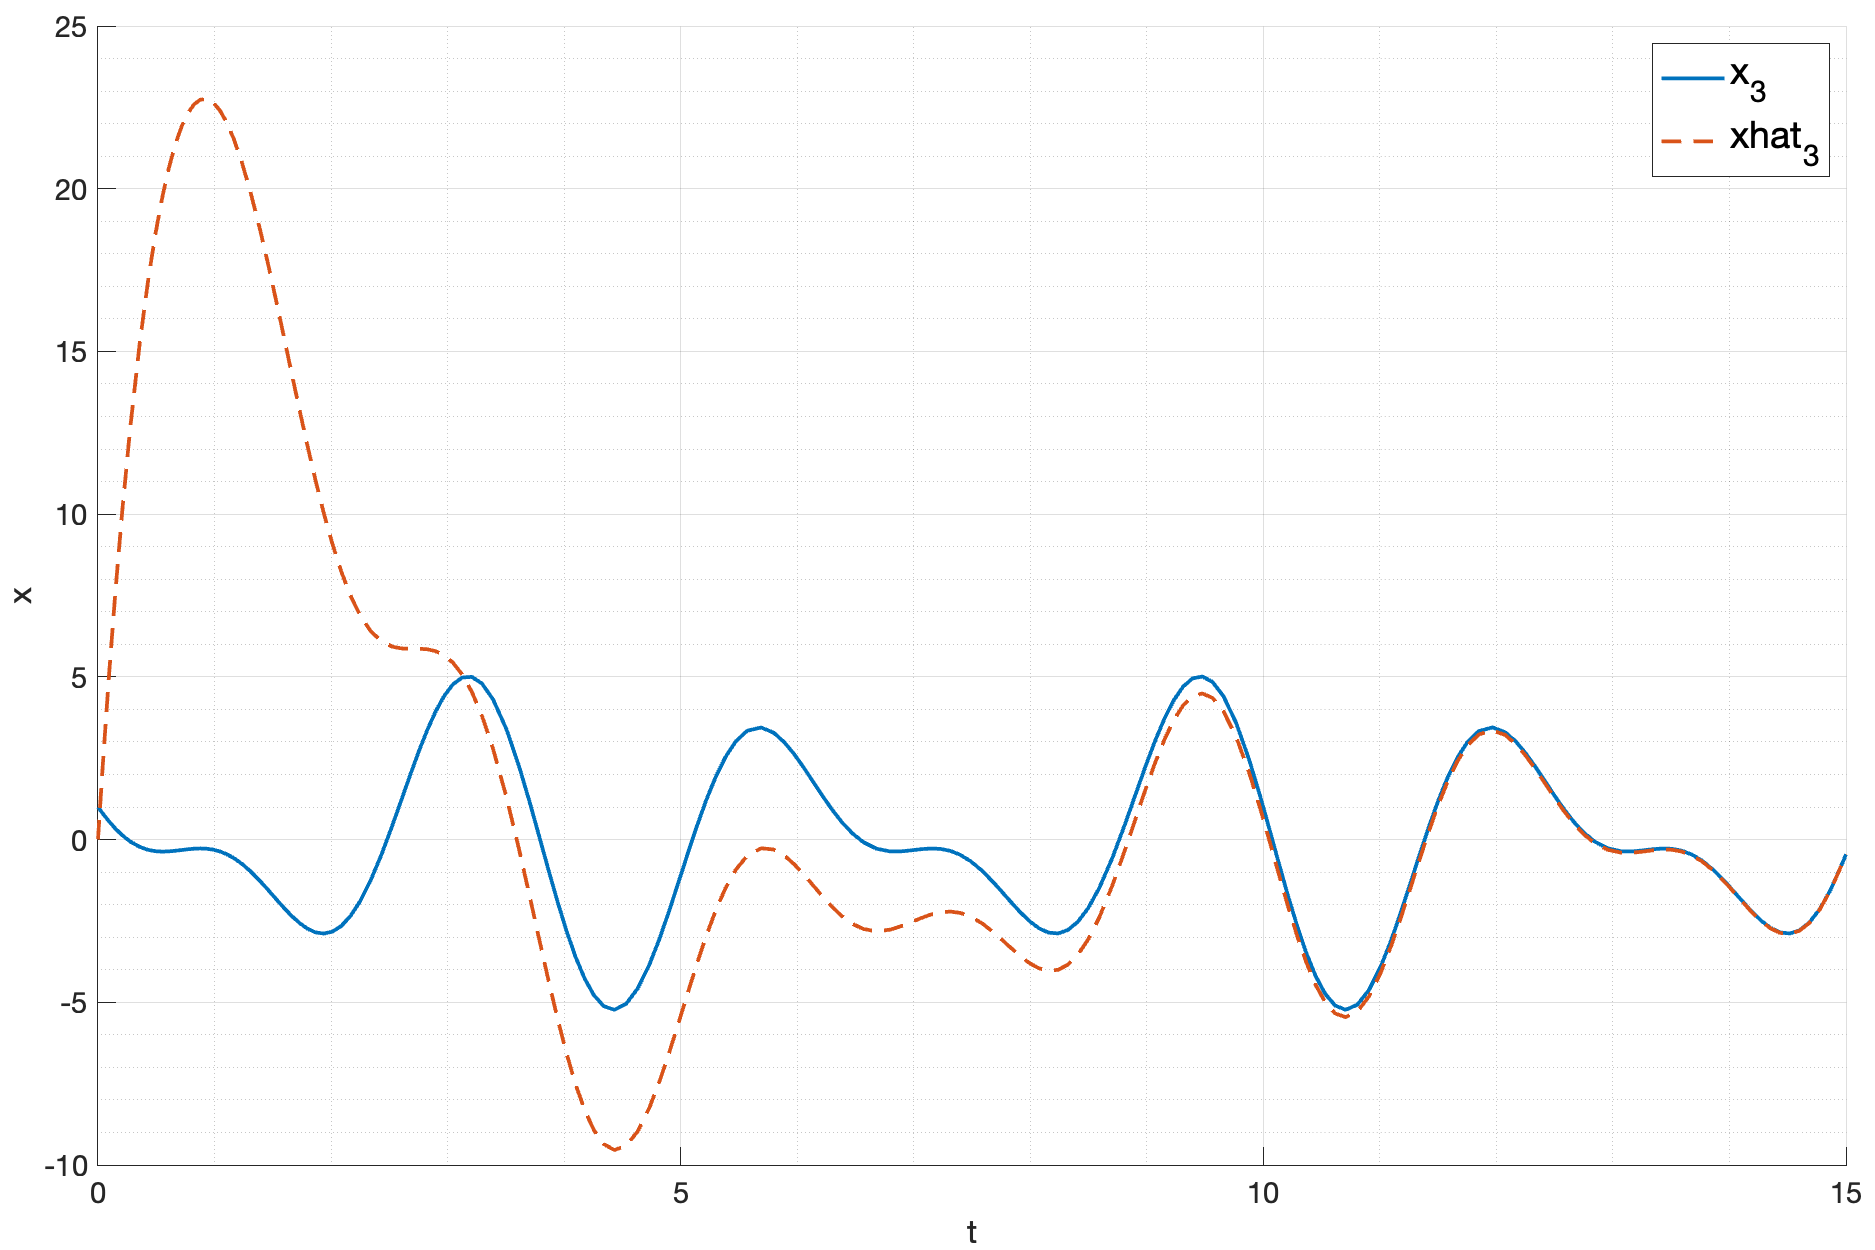
\includegraphics[width=\textwidth]{media/plots/task2_x3_1.png}
    \caption{Состояние системы $x_3$ с наблюдателем полного порядка для спектра $\sigma_1$}
    \label{fig:task2_x3_1}
\end{figure}

\begin{figure}[ht!]
    \centering
    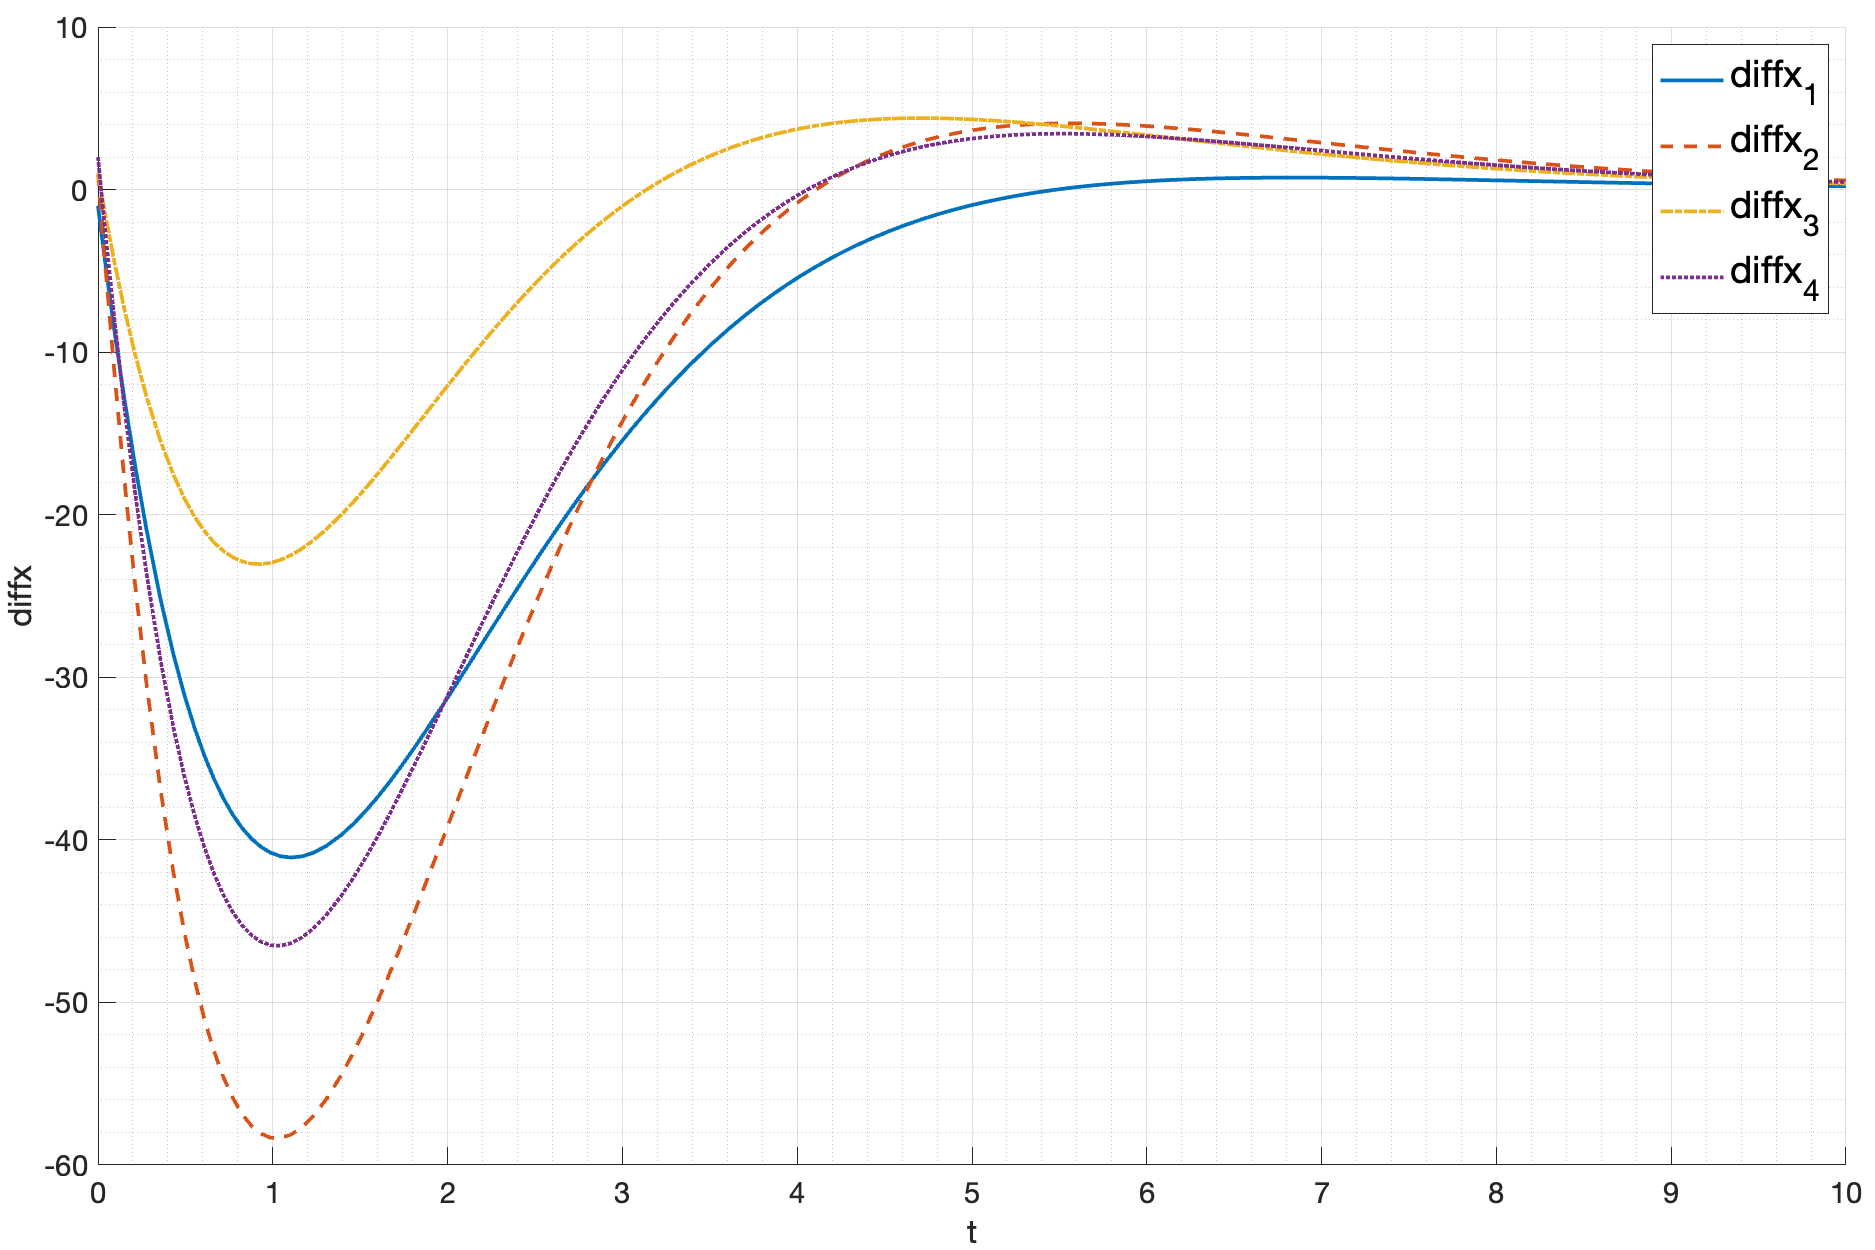
\includegraphics[width=\textwidth]{media/plots/task2_diffx_1.png}
    \caption{Ошибка наблюдателя полного порядка для спектра $\sigma_1$}
    \label{fig:task2_diff_1}
\end{figure}


Результаты моделирования для второго спектра $\sigma_2$ представлены на рисунках \ref{fig:task2_x1_2}, \ref{fig:task2_x2_2}, \ref{fig:task2_x3_2} (состояния системы), и \ref{fig:task2_diff_2} (ошибка наблюдателя).
\begin{figure}[ht!]
    \centering
    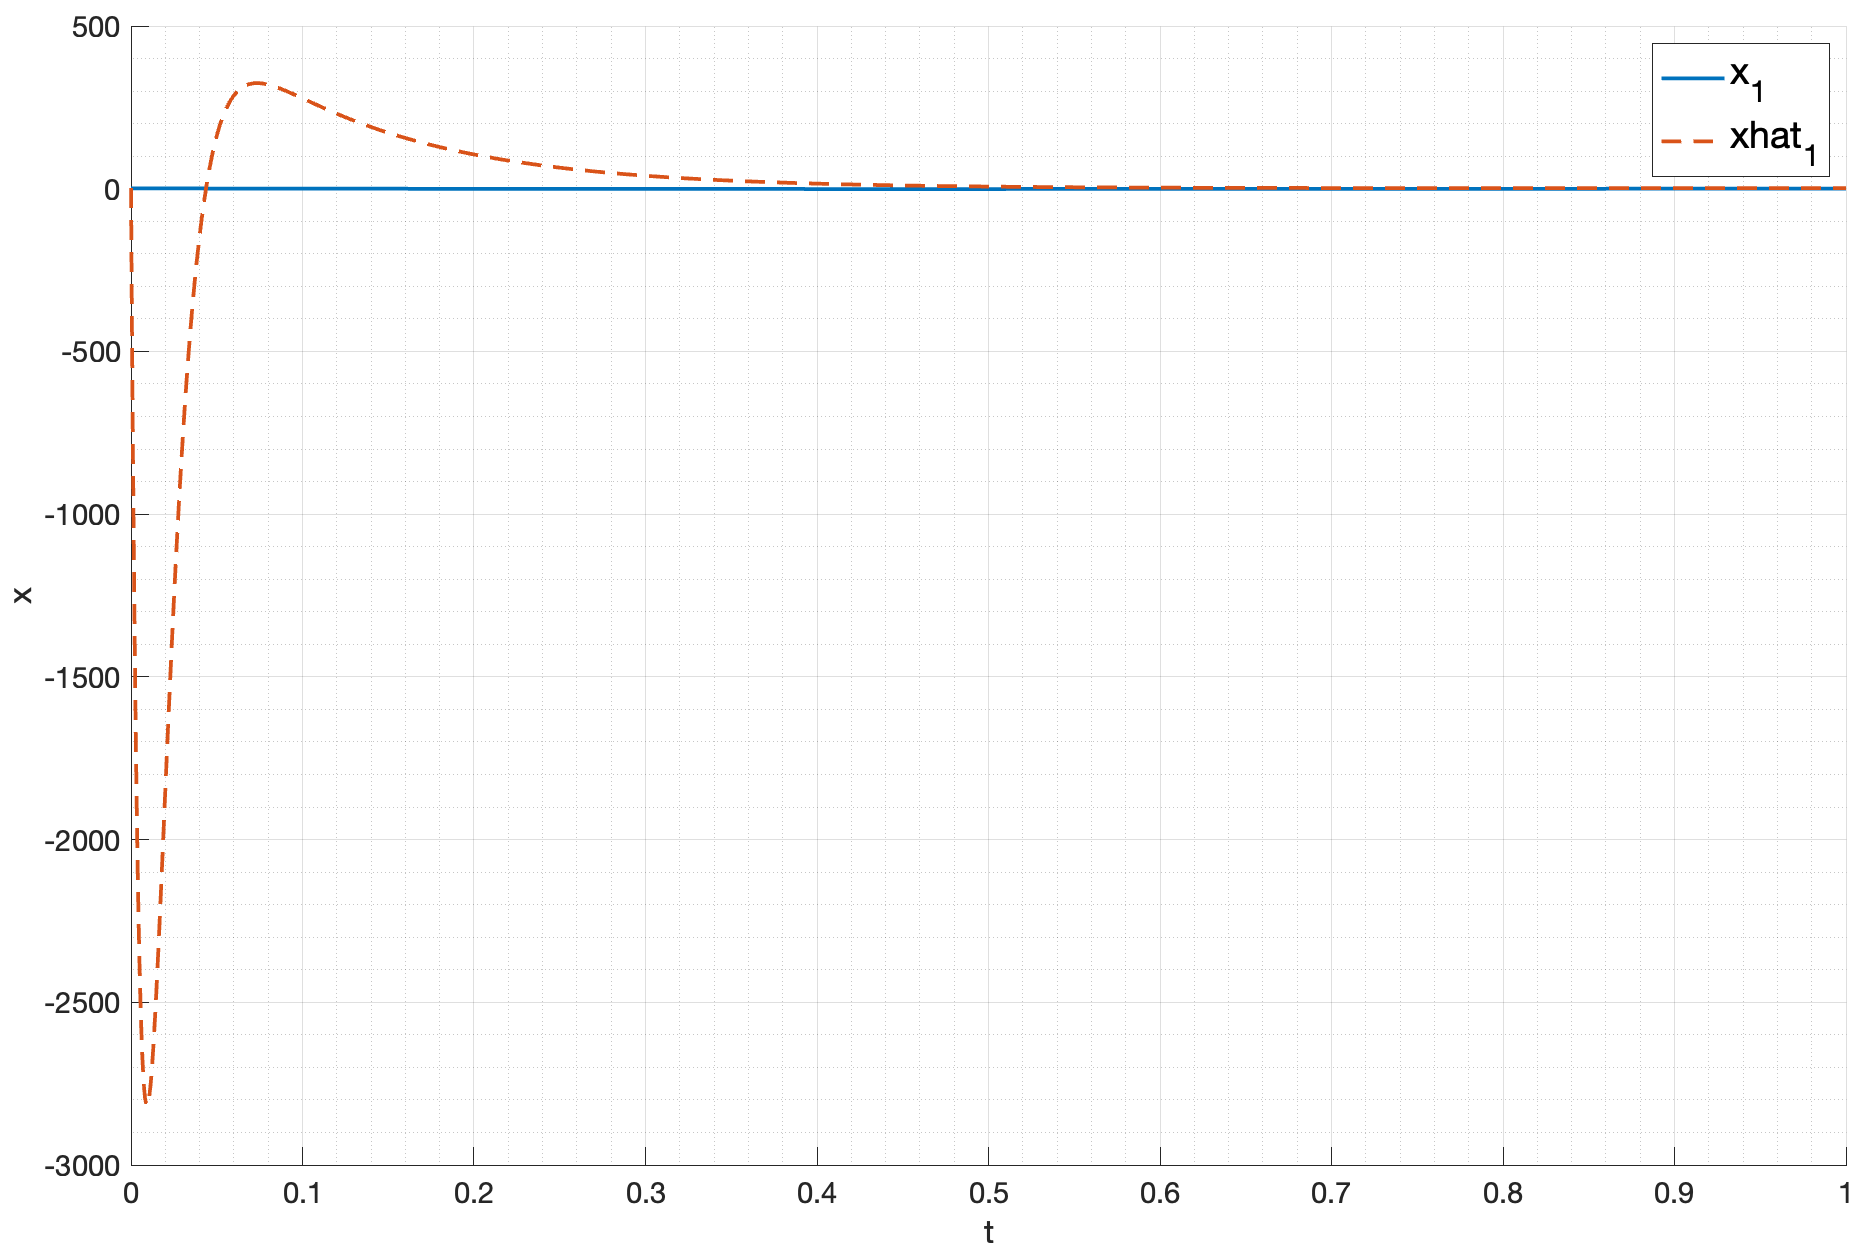
\includegraphics[width=\textwidth]{media/plots/task2_x1_2.png}
    \caption{Состояние системы $x_1$ с наблюдателем полного порядка для спектра $\sigma_2$}
    \label{fig:task2_x1_2}
\end{figure}

\begin{figure}[ht!]
    \centering
    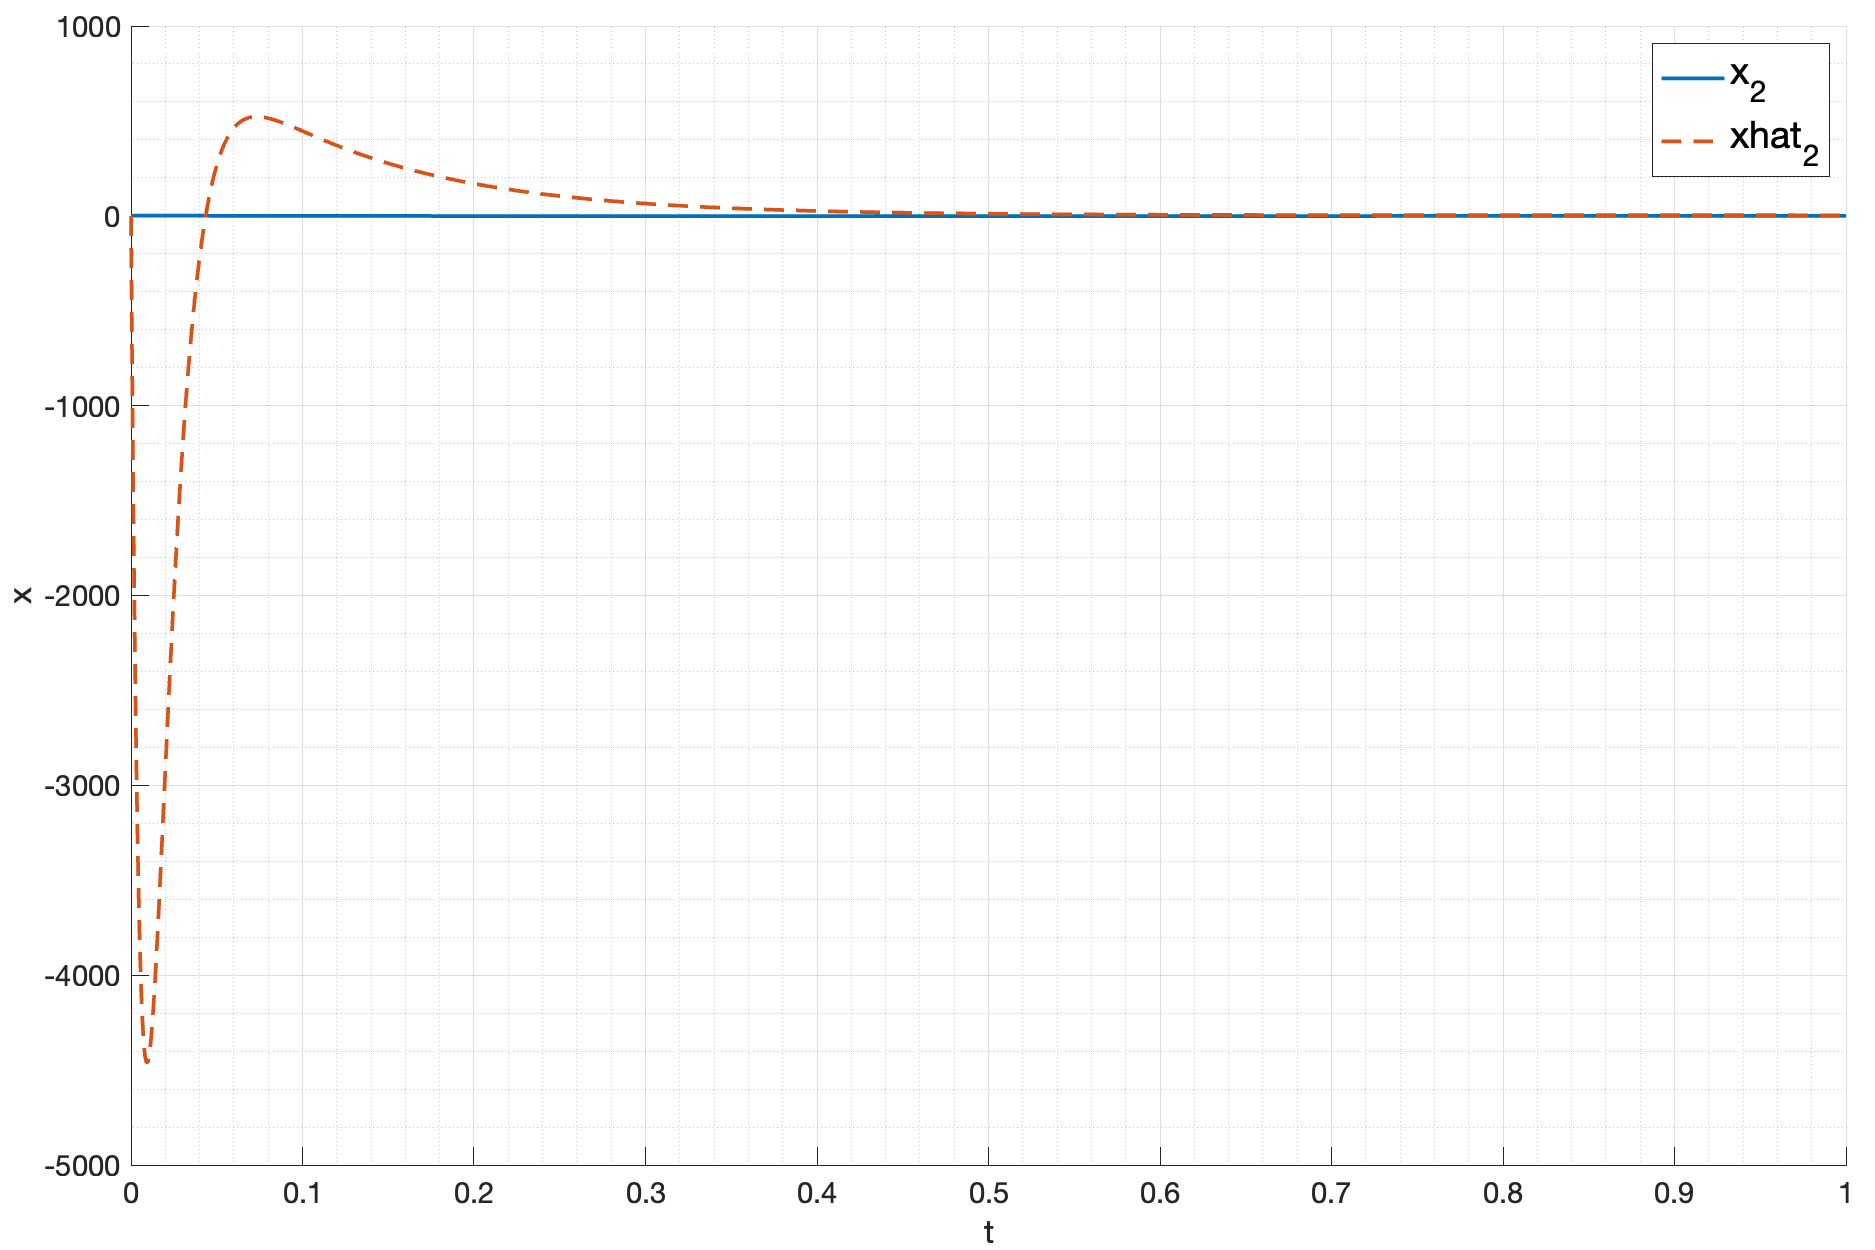
\includegraphics[width=\textwidth]{media/plots/task2_x2_2.png}
    \caption{Состояние системы $x_2$ с наблюдателем полного порядка для спектра $\sigma_2$}
    \label{fig:task2_x2_2}
\end{figure}

\begin{figure}[ht!]
    \centering
    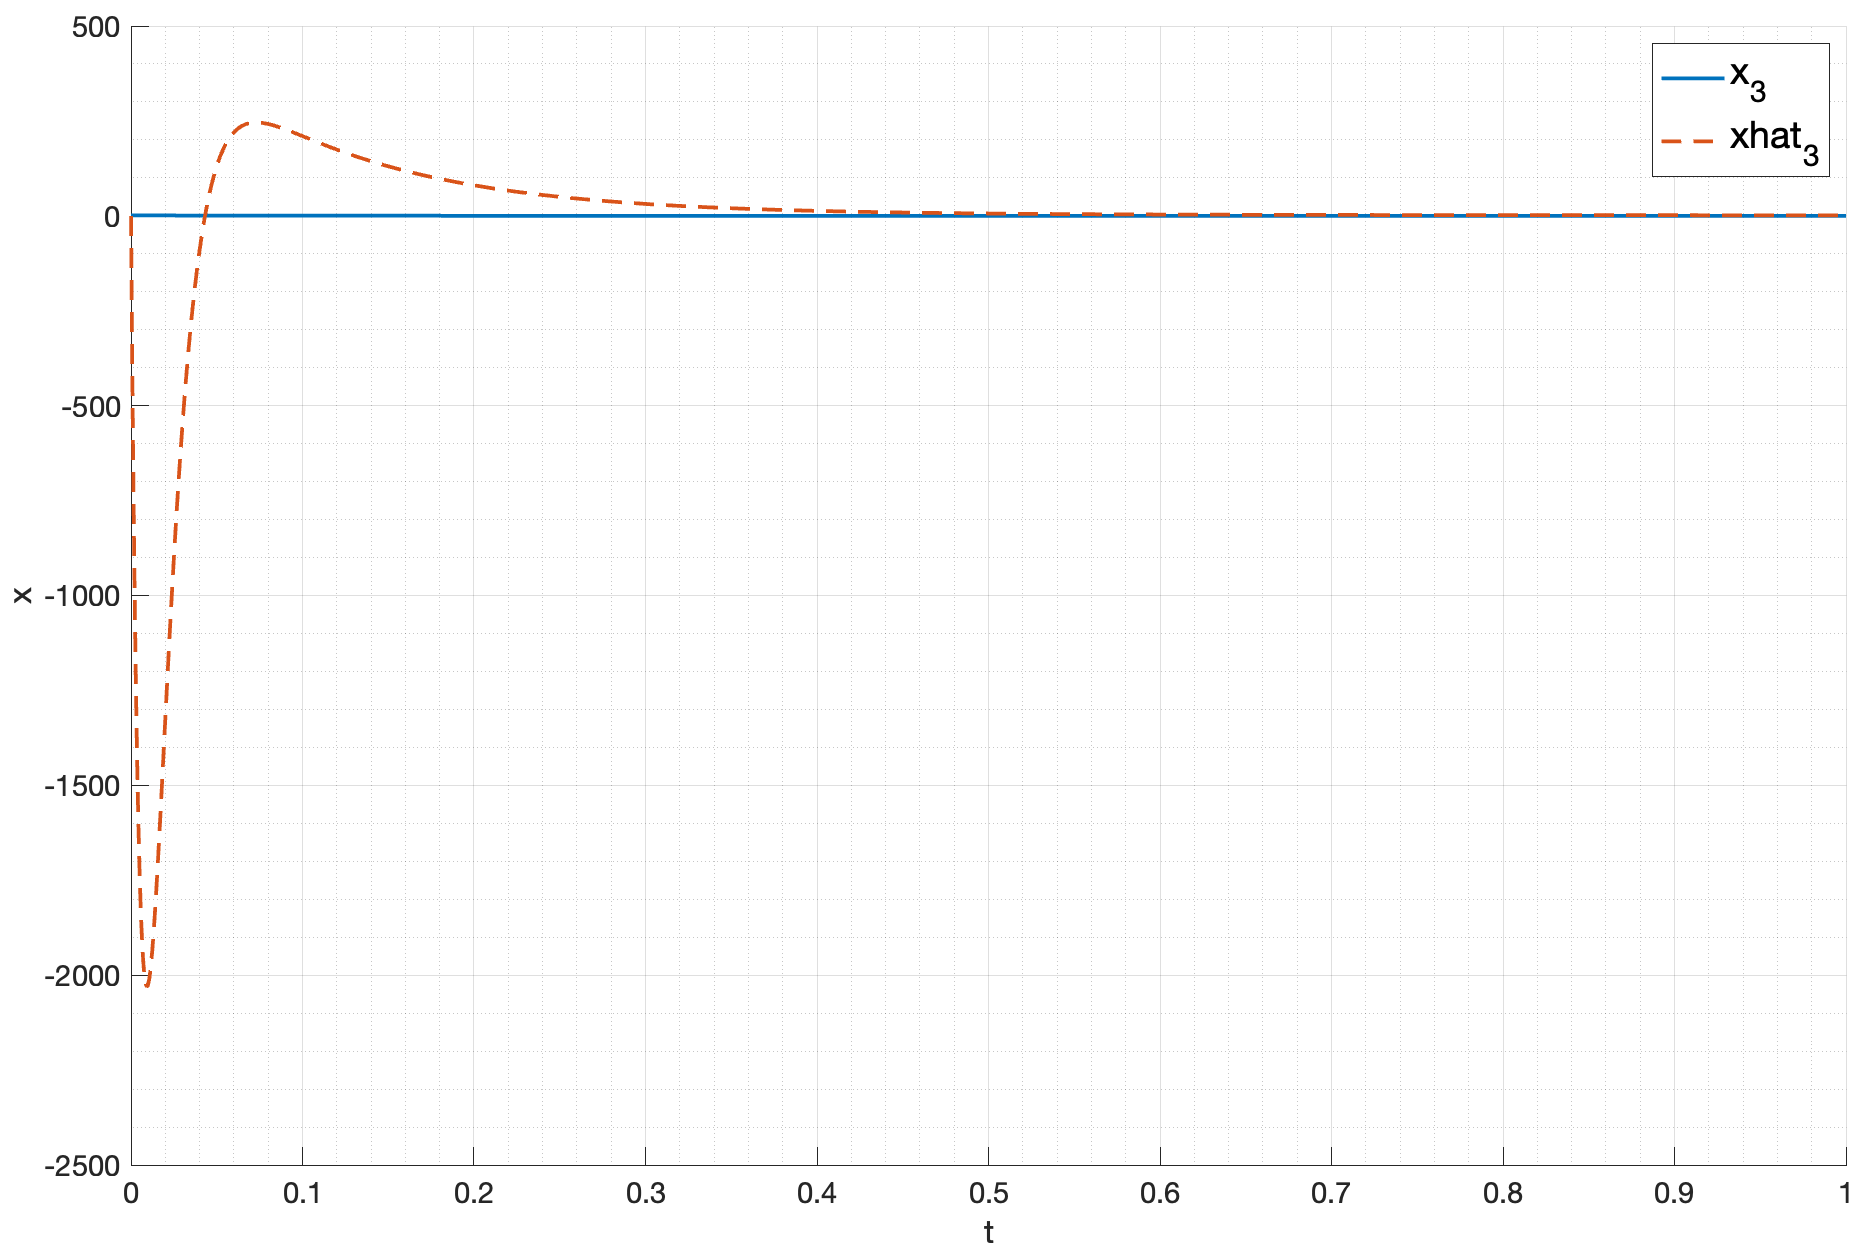
\includegraphics[width=\textwidth]{media/plots/task2_x3_2.png}
    \caption{Состояние системы $x_3$ с наблюдателем полного порядка для спектра $\sigma_2$}
    \label{fig:task2_x3_2}
\end{figure}

\begin{figure}[ht!]
    \centering
    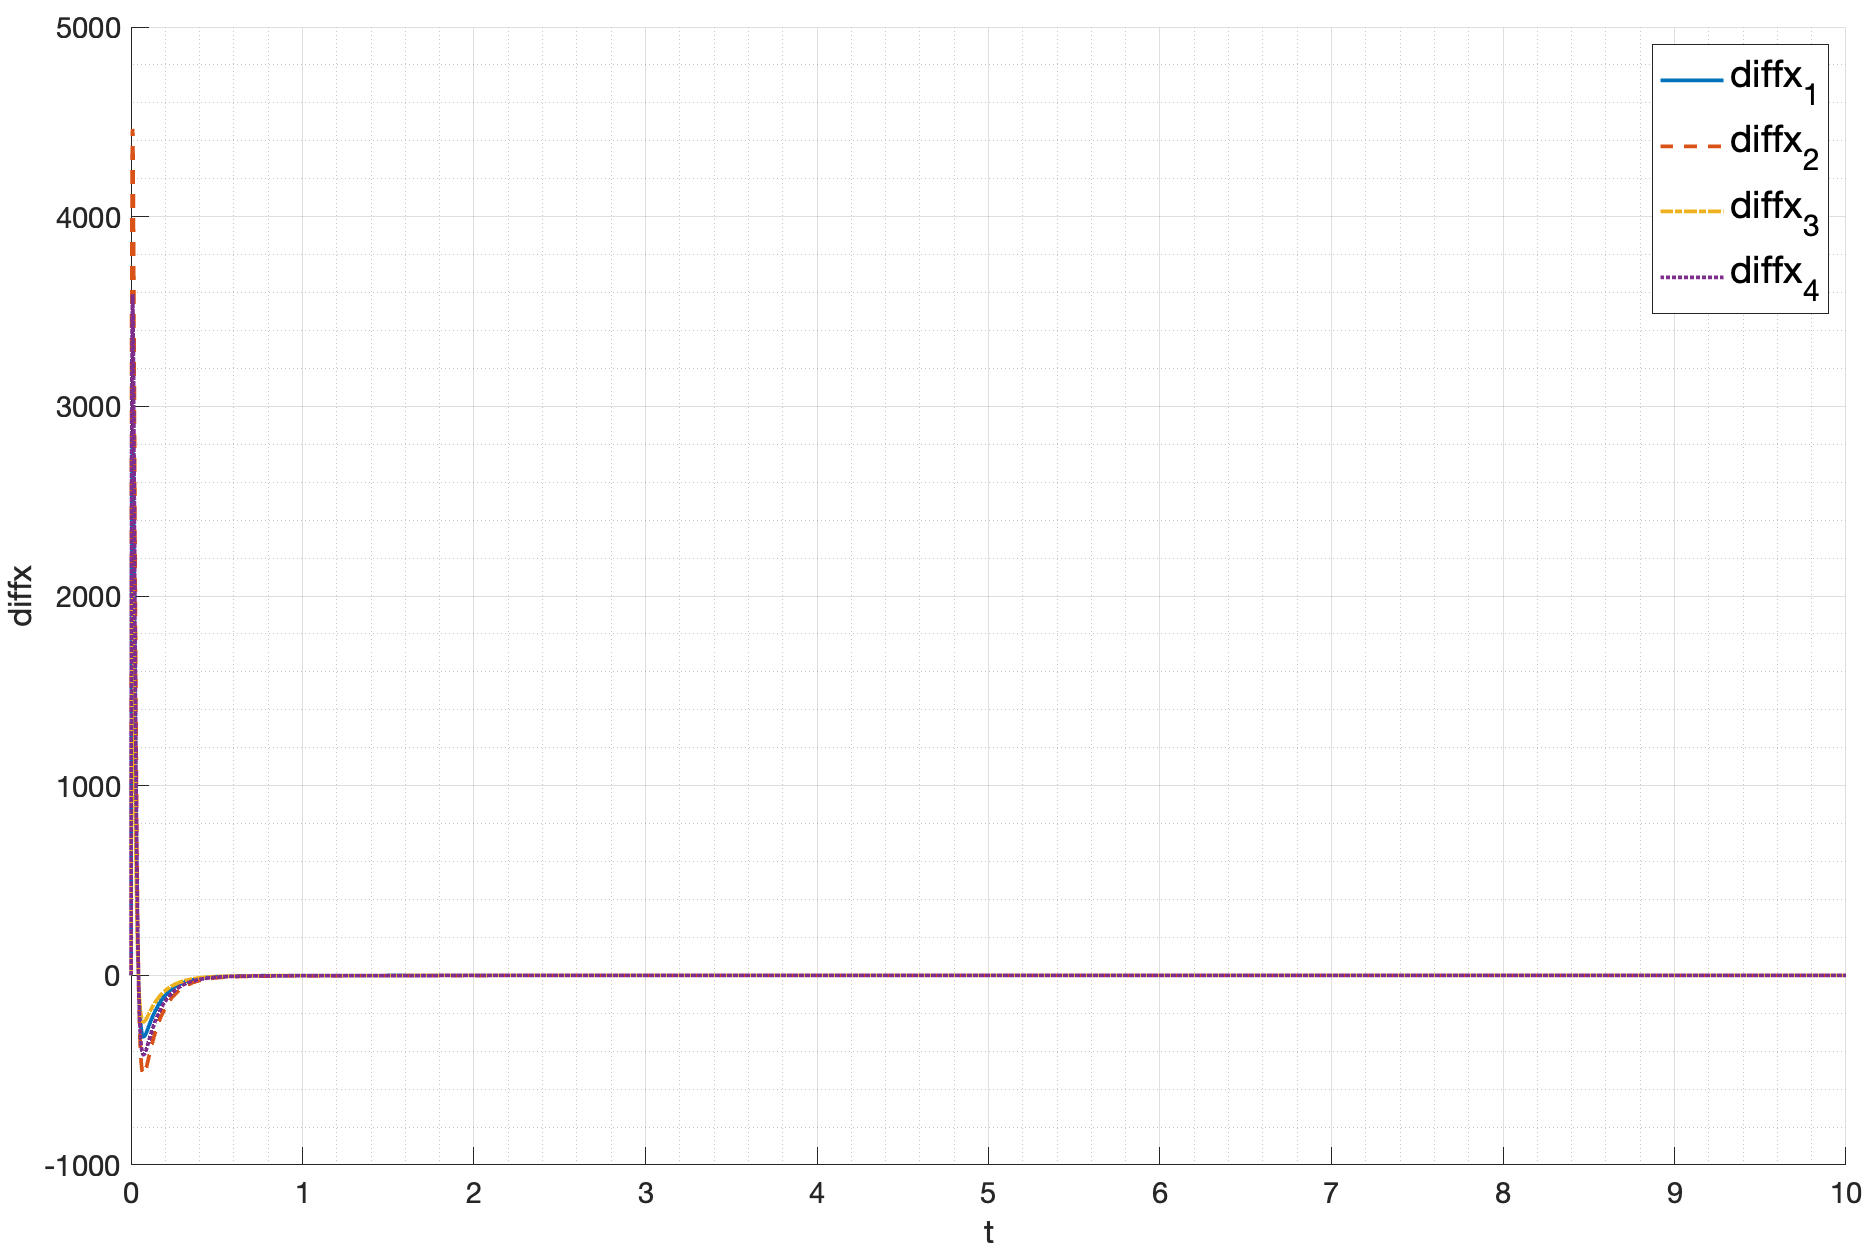
\includegraphics[width=\textwidth]{media/plots/task2_diffx_2.png}
    \caption{Ошибка наблюдателя полного порядка для спектра $\sigma_2$}
    \label{fig:task2_diff_2}
\end{figure}

Результаты моделирования для третьего спектра $\sigma_3$ представлены на рисунках \ref{fig:task2_x1_3}, \ref{fig:task2_x2_3}, \ref{fig:task2_x3_3} (состояния системы), и \ref{fig:task2_diff_3} (ошибка наблюдателя).
\begin{figure}[ht!]
    \centering
    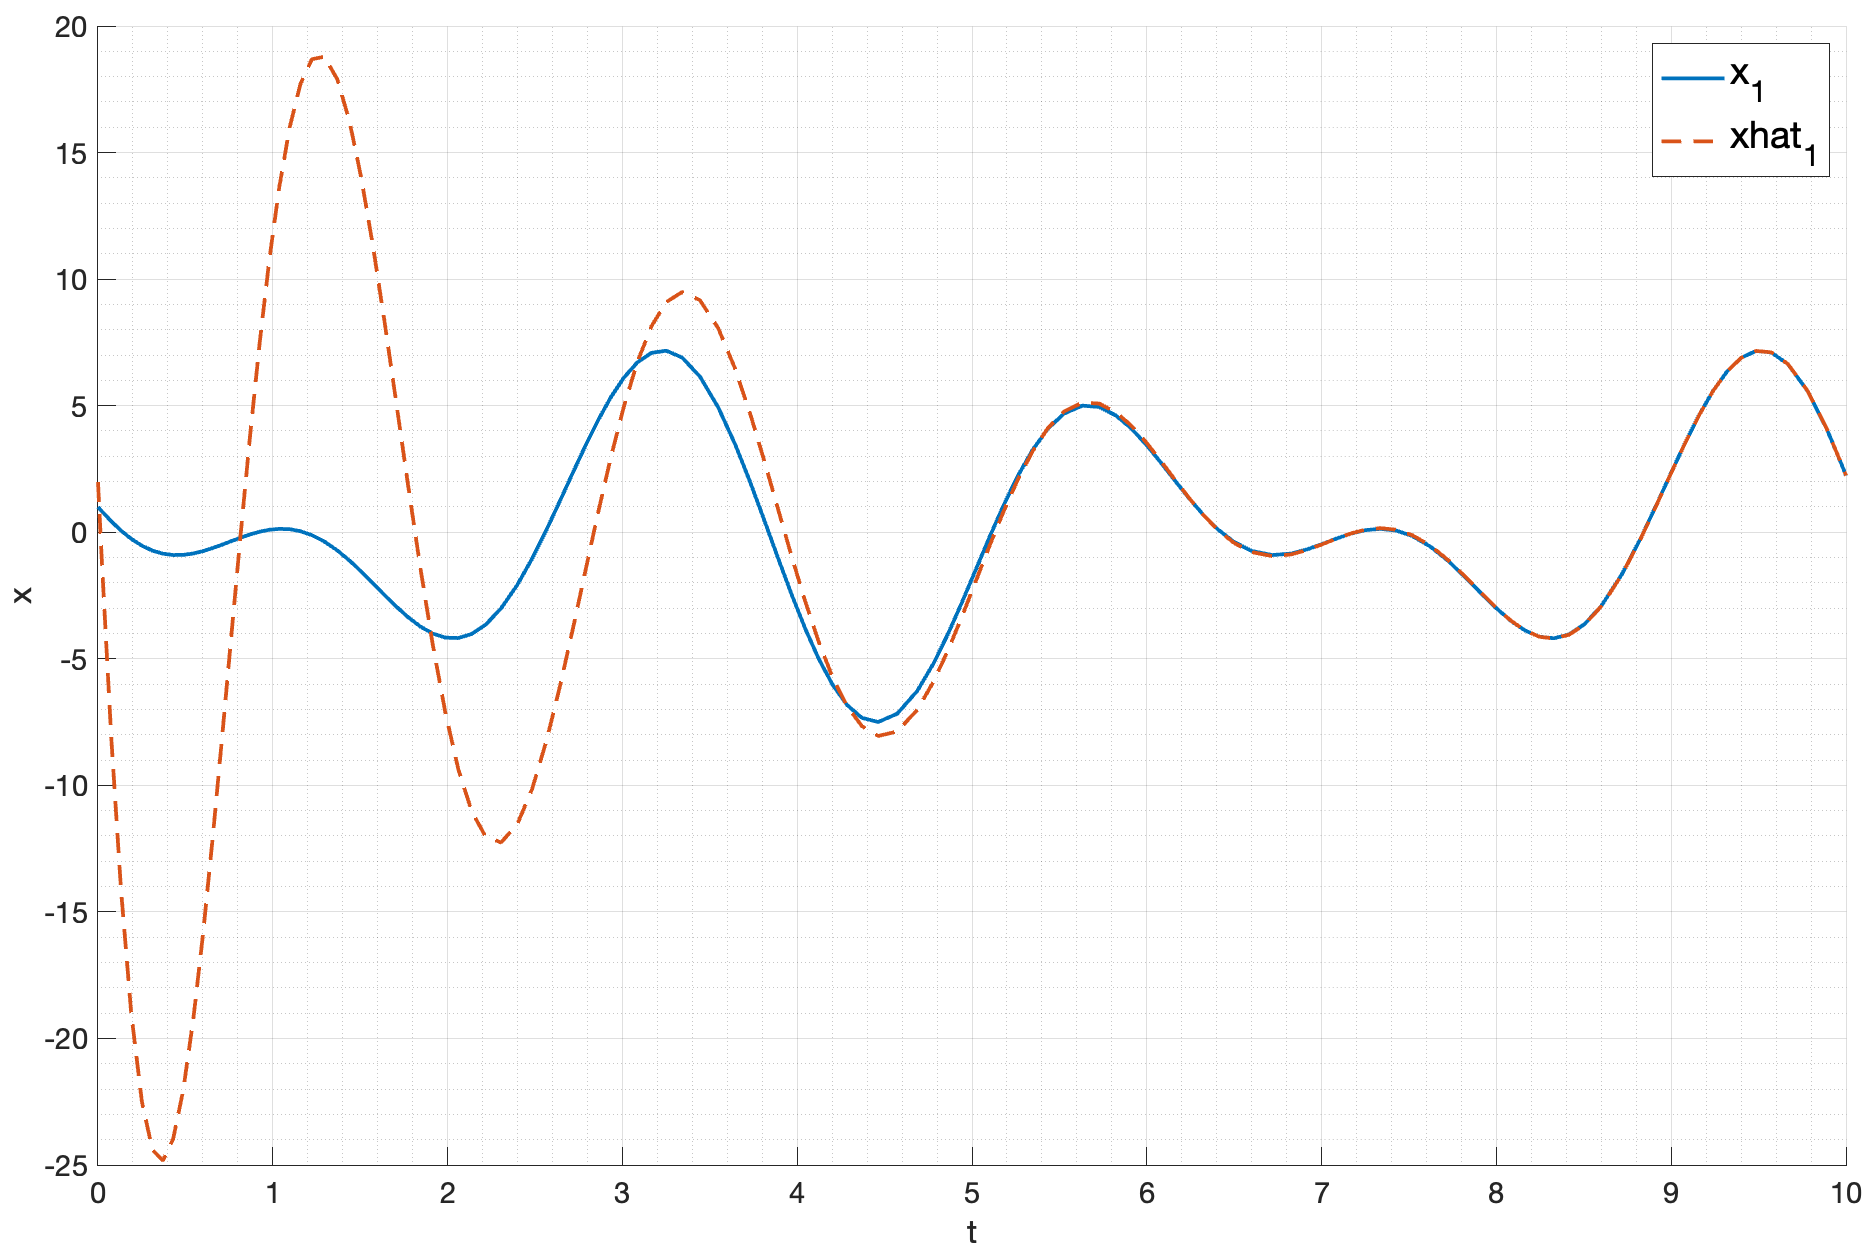
\includegraphics[width=\textwidth]{media/plots/task2_x1_3.png}
    \caption{Состояние системы $x_1$ с наблюдателем полного порядка для спектра $\sigma_3$}
    \label{fig:task2_x1_3}
\end{figure}

\begin{figure}[ht!]
    \centering
    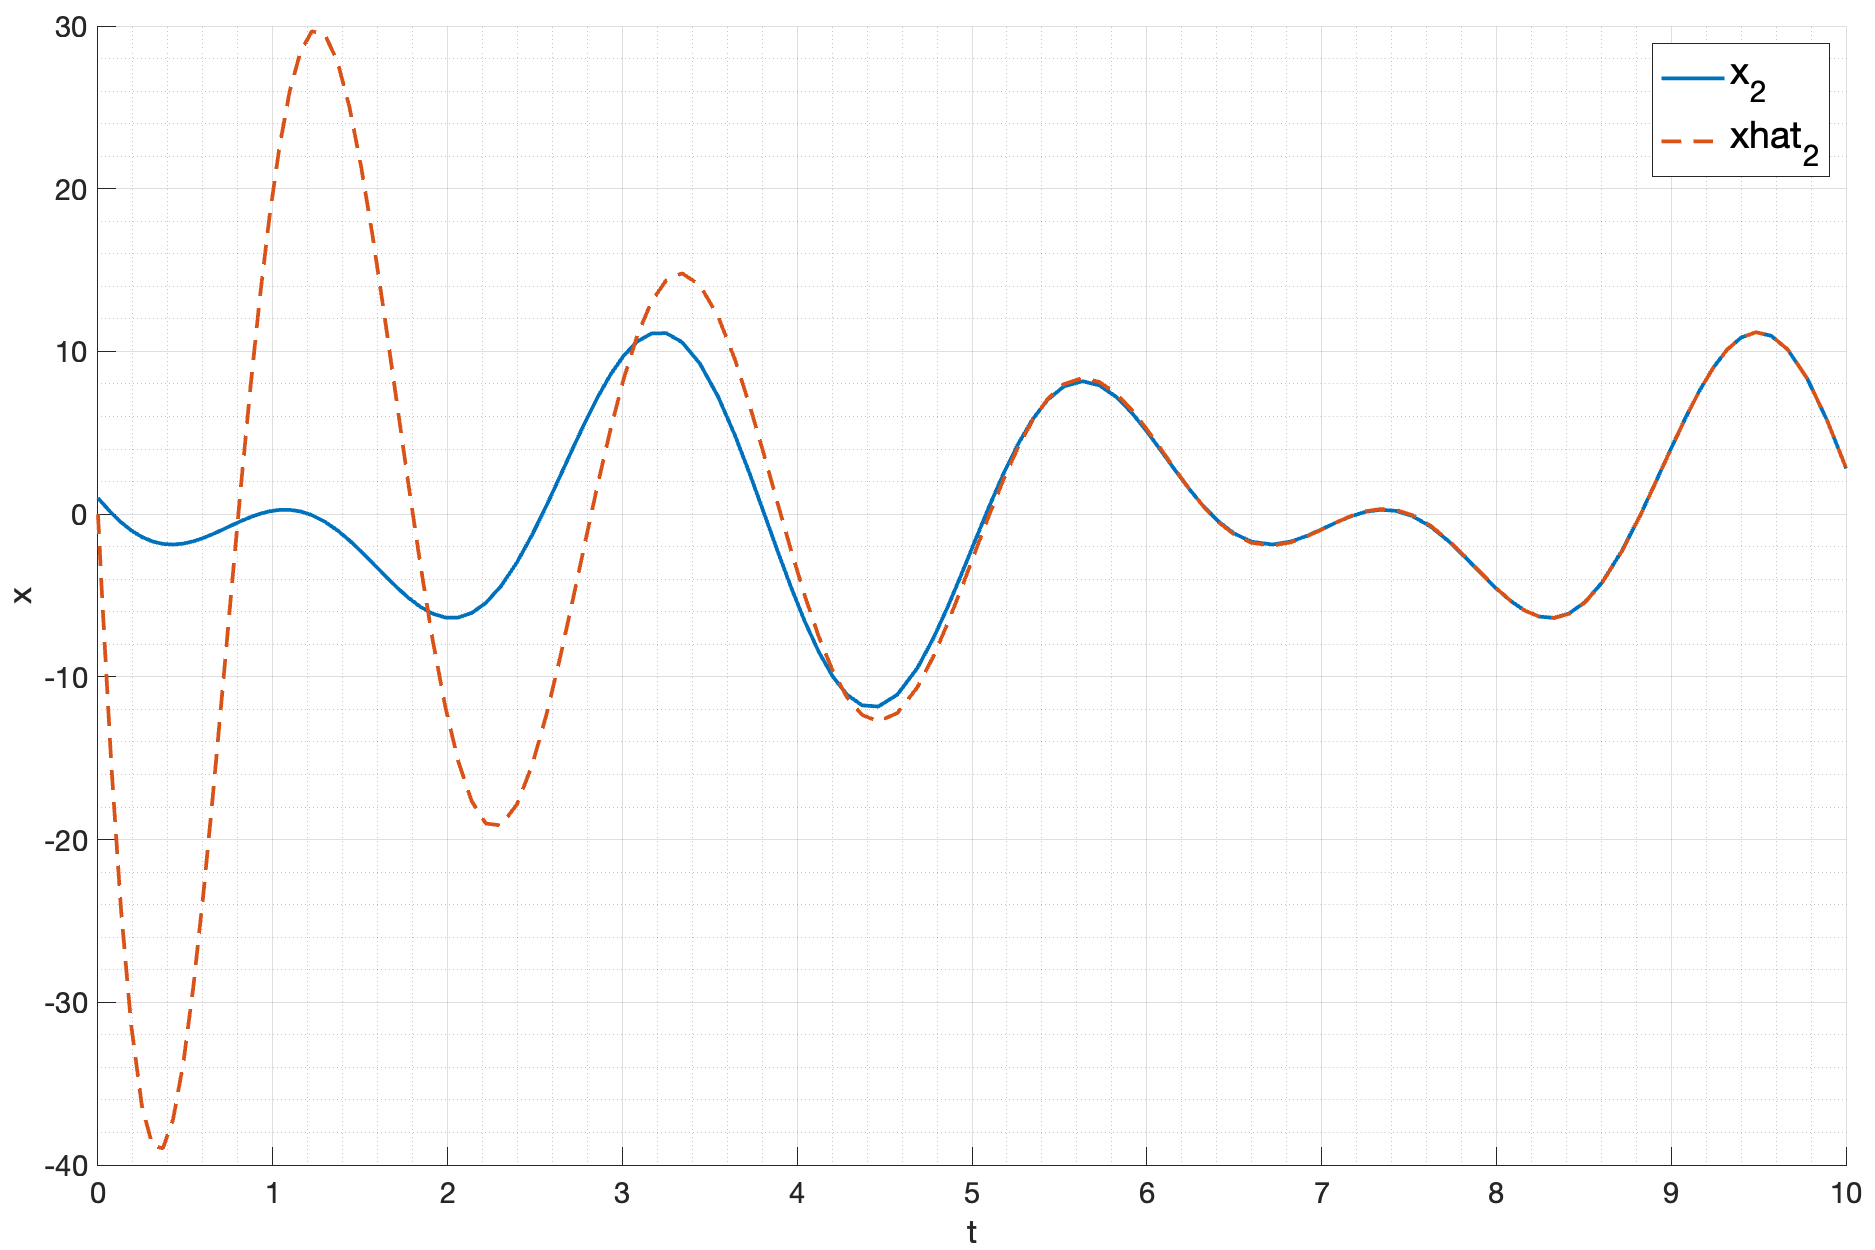
\includegraphics[width=\textwidth]{media/plots/task2_x2_3.png}
    \caption{Состояние системы $x_2$ с наблюдателем полного порядка для спектра $\sigma_3$}
    \label{fig:task2_x2_3}
\end{figure}

\begin{figure}[ht!]
    \centering
    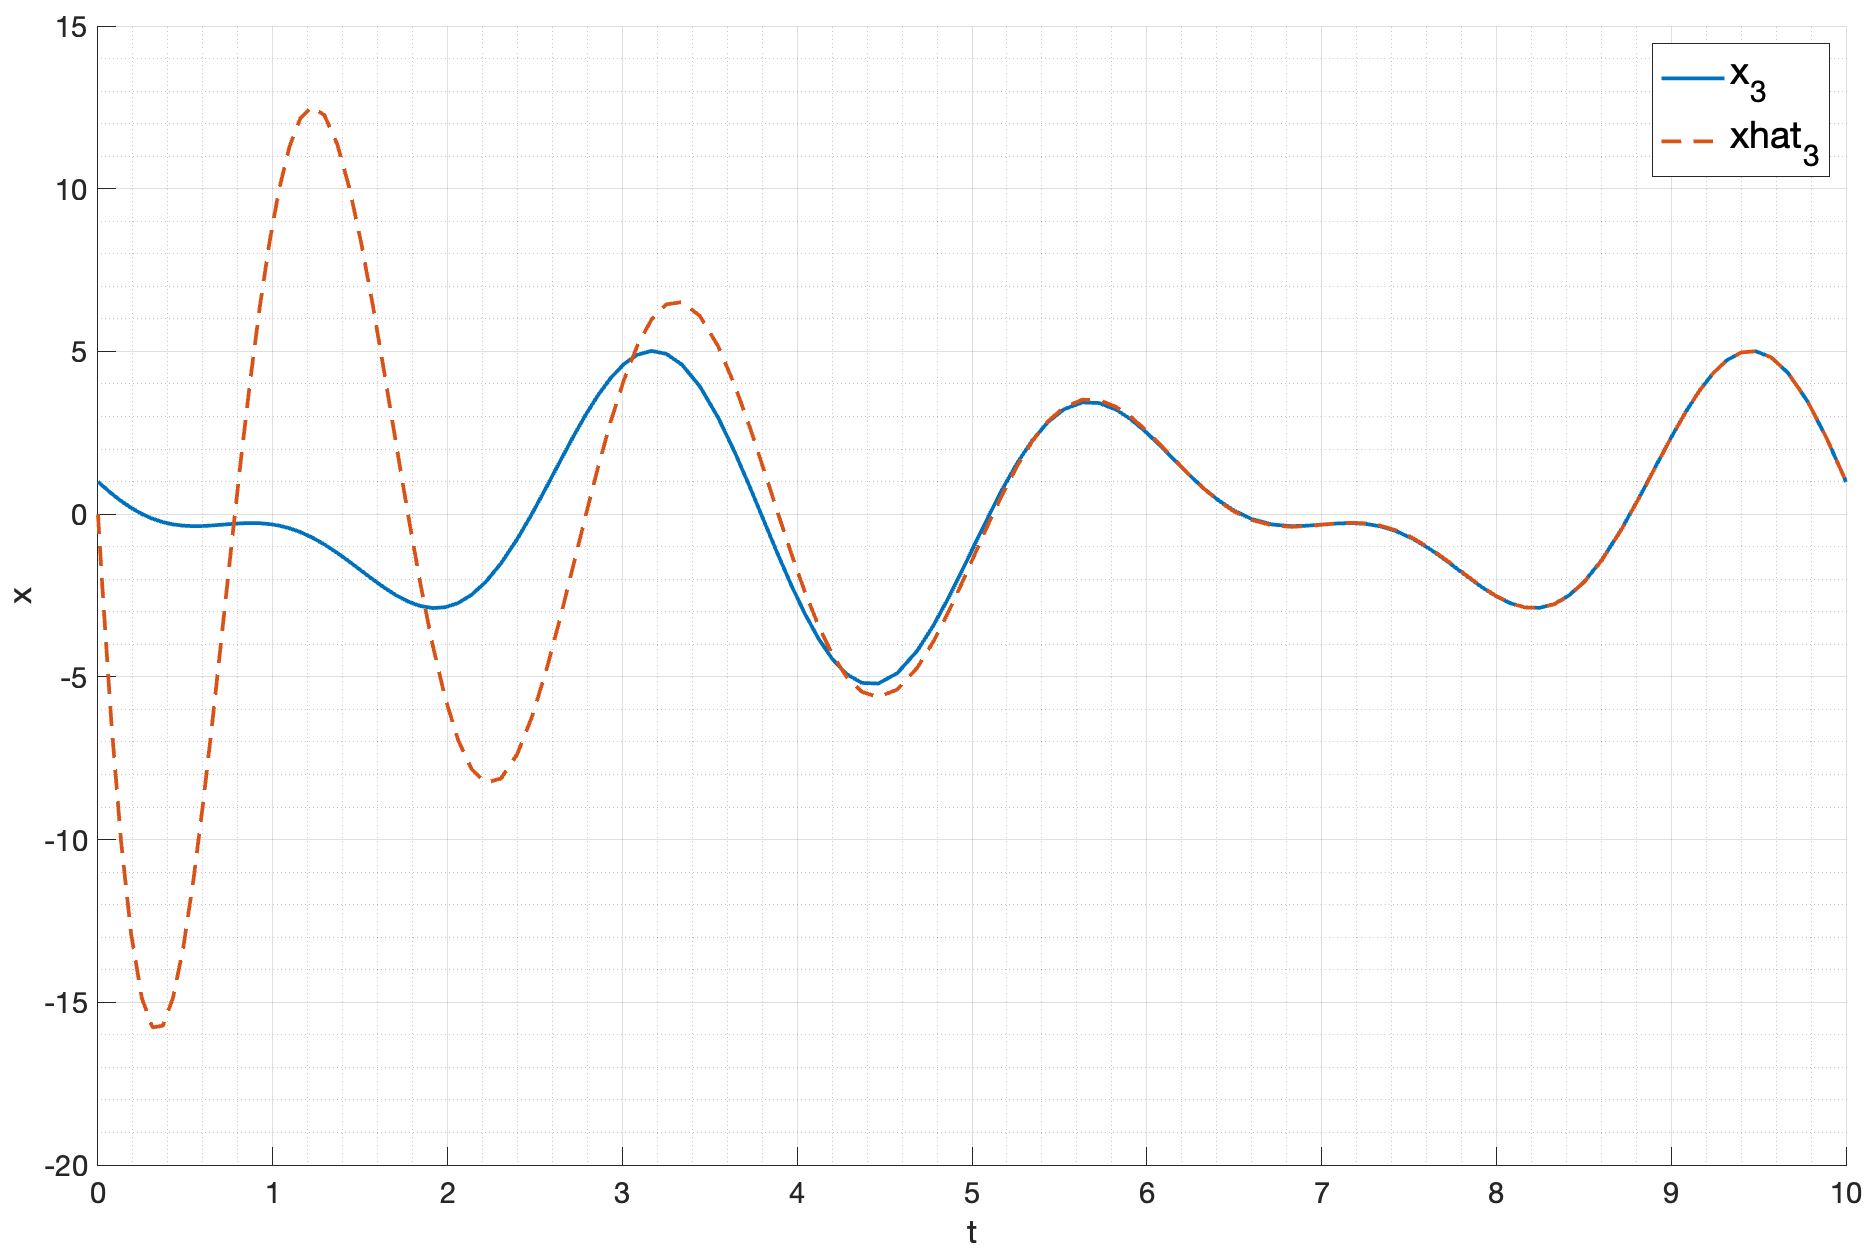
\includegraphics[width=\textwidth]{media/plots/task2_x3_3.png}
    \caption{Состояние системы $x_3$ с наблюдателем полного порядка для спектра $\sigma_3$}
    \label{fig:task2_x3_3}
\end{figure}

\begin{figure}[ht!]
    \centering
    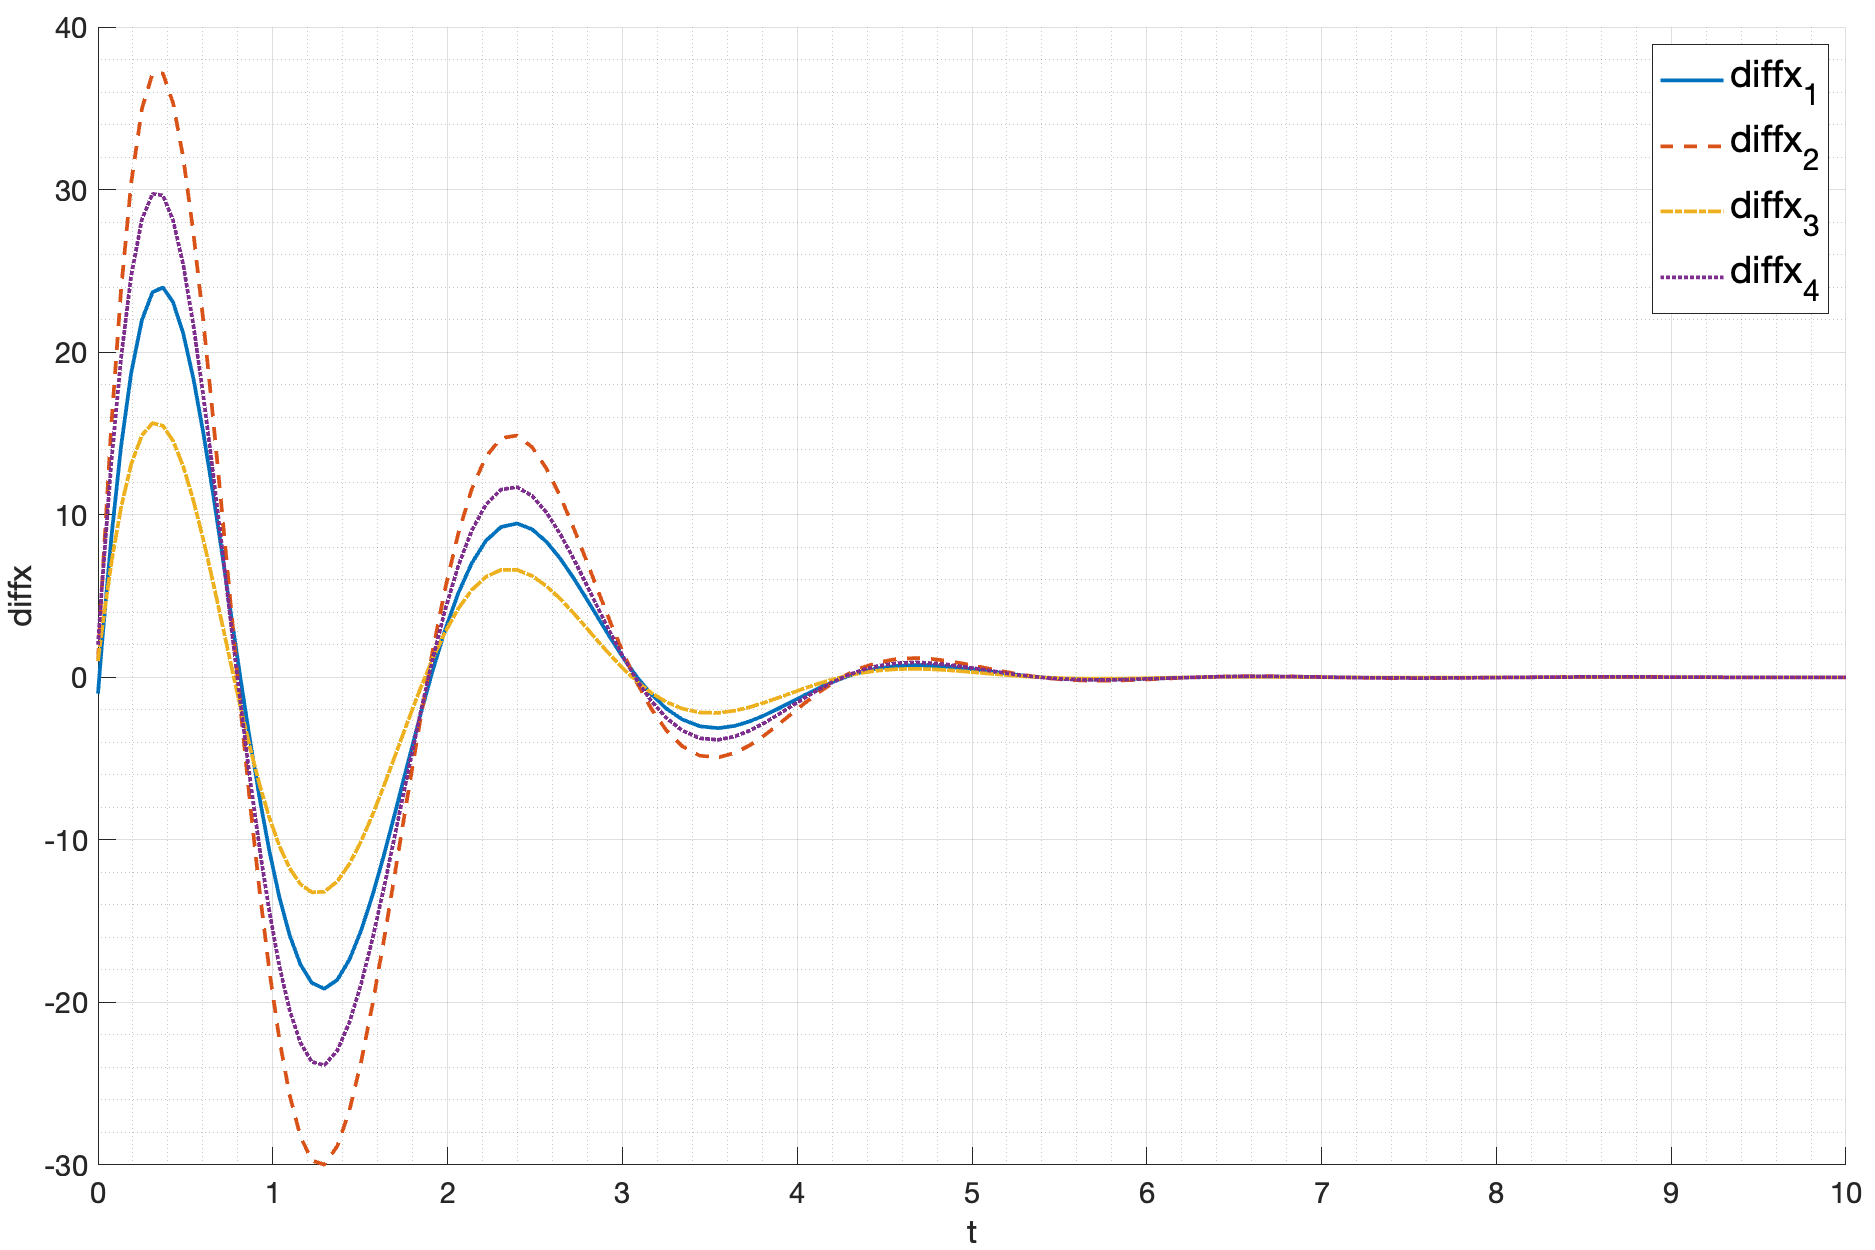
\includegraphics[width=\textwidth]{media/plots/task2_diffx_3.png}
    \caption{Ошибка наблюдателя полного порядка для спектра $\sigma_3$}
    \label{fig:task2_diff_3}
\end{figure}

\FloatBarrier
\subsection{Выводы}
Во всех случаях коррекция наблюдателя помогла устремить ошибку к нулю. При этом, как и в прошлом задании, 
можно заметить закономерность. При больших значениях спектра наблюдателя ошибка устремляется к нулю быстрее, чем при малых, 
а при наличии комплексных собственных чисел ошибка наблюдателя приобретает колебательный характер.